\chapter{Validation of WARP3D Results with Experimental Data} \label{chap:experiment-validation}

% Here we find some existing results and compare them to what can be modeled.

One of the goals of this research is to provide easier validation of EPFM experiments in ASTM E2219.
The standard requires the construction of an elastic-plastic finite element model, with geometry and material properties matching those used in the experiment.
Though the work presented in \Cref{chap:abaqus-validation} demonstrates the consistency of two independent finite element solutions along most of the crack front, the numerical results need to be compared to experimental data to ensure real-world accuracy and applicability of results.

Raw data from a bend test of a surface-cracked plate conducted in 2010 was obtained from Dr. Phillip Allen of NASA MSFC.
The test data was compared to the results from a purpose-built finite element model where dimensions and material properties were matched wherever possible, and then to interpolated results using existing database values for dimensions and material properties.
The test specimen had cross-sectional dimensions of \(W_\text{test}=3.00\)~inch and \(t_\text{test}=0.374\)~inch, crack dimensions of \(a_\text{test}=0.215\)~inch, \(2c_\text{test}=0.490\)~inch, and roller span distances of \(S_\text{outer,test}=10.168\)~inch and \(S_\text{inner,test}=4.00\)~inch.
The specimen material was Aluminum 2219-T87, with \(E_\text{test}=10800\)~ksi, \(\nu_\text{test}=0.3\), \(\sigma_\text{ys,test}=56.0\)~ksi, and \(n_\text{test}=9\).
Test data gathered included applied load and CMOD.
% Not sure if this is the real experiment or not. Was in PPT, but doesn't look like a four-point.
%A photo of the experimental setup can be seen in \Cref{fig:bend_test}.
%
%\begin{figure}[tbp]
%\centering
%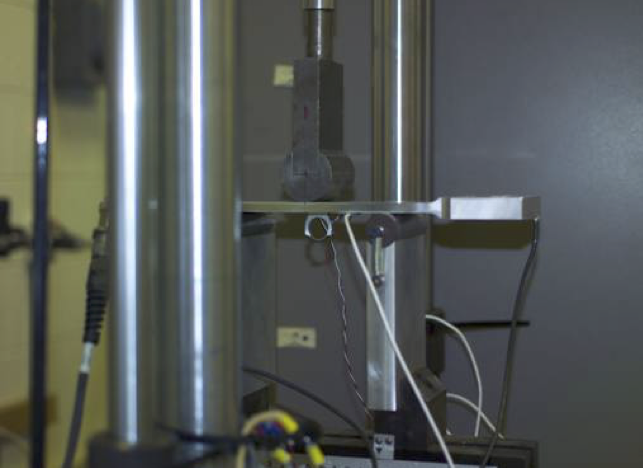
\includegraphics[width=0.8\columnwidth]{nasa-bend-test}
%\caption{\label{fig:bend_test} NASA bend test used for experimental validation}
%\end{figure}

\section{Validation of Purpose-Built Model Results}
\label{sec:validation-purpose-built}

% Step 1, build FEACrack model of correct geometry and material properties (no interpolation). Use that to validate.

The programs and procedures developed in \Cref{chap:development-bending-models} were used to create a WARP3D input file, with \(\frac{a}{c}=0.878\), \(\frac{a}{t}=0.575\), \(\frac{E}{\Sys}=192.3\), \(n=9\), and \(\Sys=53.05\)~ksi.
The default values of \(W\), \(\Sinner\), and \(\Souter\) were used.
These values do not match the ones used in the experiment, but if comparisons are limited to CMOD values and remote bending stresses, it is trivial to adjust experimental load values to equivalent bending stresses.
An overall view of the finite element mesh is shown in \Cref{fig:exp_validation_mesh}, and details of the mesh of the crack front is shown in \Cref{fig:exp_validation_mesh_zoomed}.
\begin{figure}[tbp]
\centering
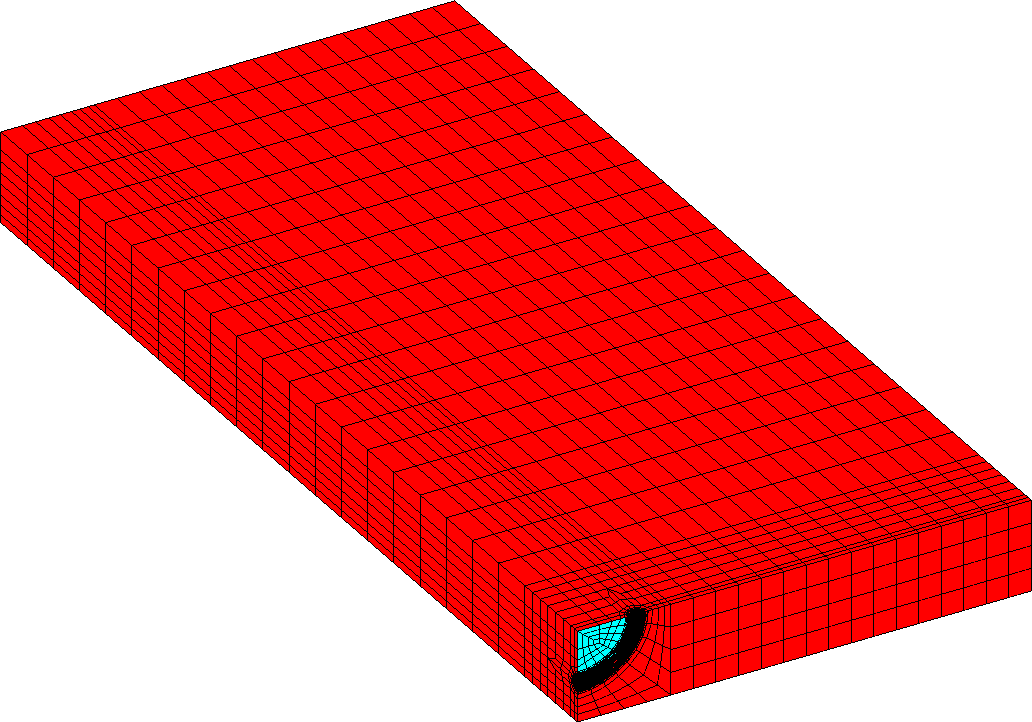
\includegraphics[width=0.8\columnwidth]{exp_validation_mesh}
\caption{\label{fig:exp_validation_mesh} Overall mesh of purpose-built experimental validation model}
\end{figure}

\begin{figure}[tbp]
\centering
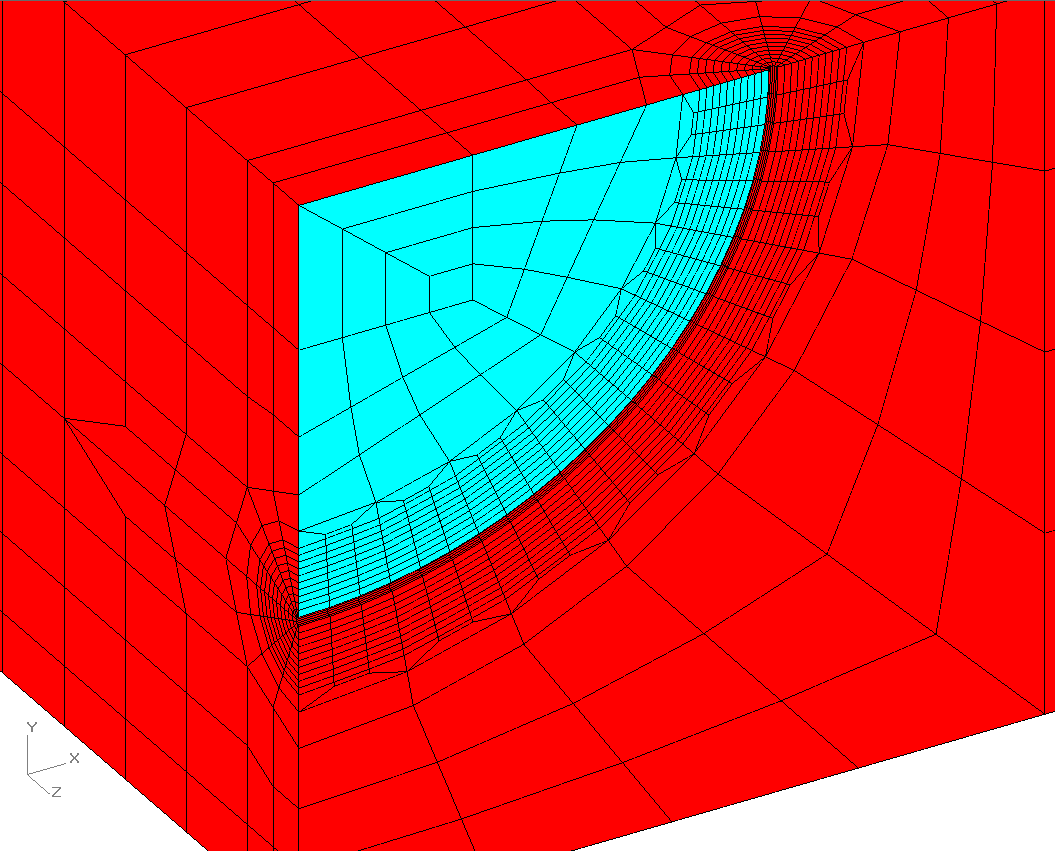
\includegraphics[width=0.8\columnwidth]{exp_validation_mesh_zoomed}
\caption{\label{fig:exp_validation_mesh_zoomed} Crack front mesh of purpose-built experimental validation model}
\end{figure}

After iteratively solving for a traction that would provide sufficient plastic deformation according to the conditions described in \Cref{sec:solve}, reaction forces, bending moments, and CMOD values were extracted from the WARP3D results.
Though reaction forces and CMOD values are easy to evaluate, additional care must be taken to accurately calculate bending moments.
Since the boundary conditions are applied to rows of nodes or faces of elements, the location of the traction and roller conditions will change as the model deforms.
This is most pronounced in the thinnest, widest plates such as the one shown in \Cref{fig:bend_ac02_at08_E0100_n03}, but occurs to some degree in all plates in bending.

For any plate model in bending, the applied bending moment can be calculated as the product of the total reaction force in the $y$ direction and the distance between the roller support and the traction plane.
Using the nomenclature of \Cref{fig:astm-e2899-4point-bend},
\begin{align}
\text{Moment} &= \frac{(\text{Reaction force})(\Souter - \Sinner)}{2}\quad,
\end{align}
where \Souter and \Sinner are no longer constant values as in a physical experiment, but are calculated by measuring the distance between the nodes where the boundary conditions are applied.

Once the applied bending moment has been calculated, maximum remote bending stresses can be calculated via mechanics of materials methods as
\begin{align}
\sigma &= \frac{(\text{Moment})(t)}{2 I_{xx}}\quad,
\end{align}
where \(I_{xx}\) is the second moment of area of the cross section with respect to the \(x\) axis.
A comparison between the experimental and numerical results is shown in \Cref{fig:exp_validation_stress_cmod}, with stress values accurate to within 2~ksi across the entire experimental range.
\begin{figure}[tbp]
\centering
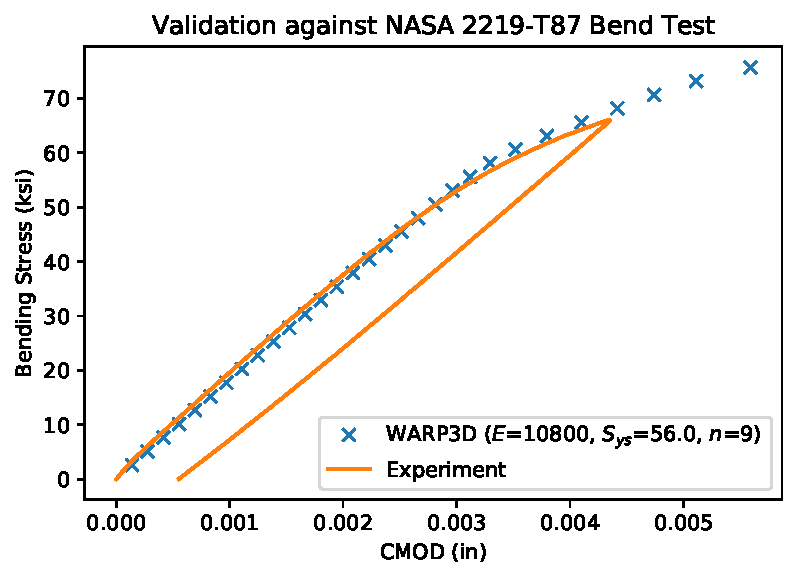
\includegraphics[width=0.8\columnwidth]{experimental-validation-stress-cmod}
\caption{\label{fig:exp_validation_stress_cmod} Comparison of bending stress and CMOD between purpose-built model and experiment}
\end{figure}
By manipulating the standard bending stress formula \(\sigma = \frac{M c}{I}\) to \(M = \frac{\sigma I}{c}\) using \(c\) and \(I\) values from the experiment, the bending moment can be predicted as shown in \Cref{fig:exp_validation_moment_cmod}.
\begin{figure}[tbp]
\centering
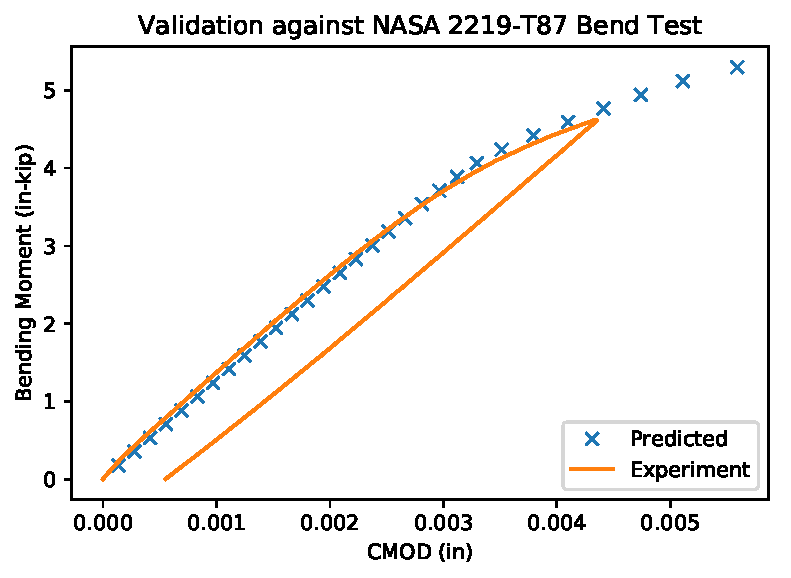
\includegraphics[width=0.8\columnwidth]{experimental-validation-moment-cmod}
\caption{\label{fig:exp_validation_moment_cmod} Comparison of predicted bending moment and CMOD between purpose-built model and experiment}
\end{figure}
The final step is to convert the predicted bending moment into a predicted applied load.
This requires scaling the moment by the total distance between the outer and inner rollers on the test, and then scaling the resulting value by a factor of 4 to account for the model reaction force being only 25\% of the equivalent experimental measure (the model reaction only covers half the length of one roller, and the experimental load is effectively distributed over two full rollers):
\[
P_\text{predicted} = \frac{4 M_\text{predicted}}{\Souter - \Sinner}
\]
\begin{figure}[tbp]
\centering
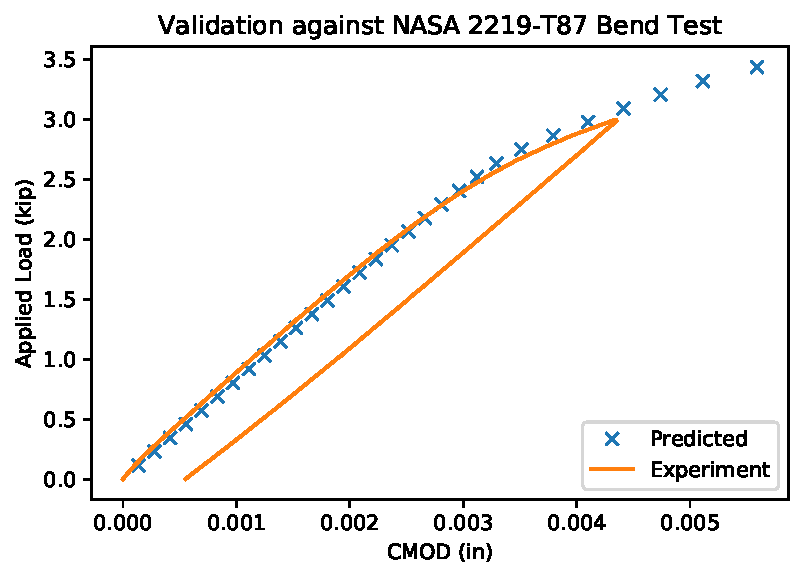
\includegraphics[width=0.8\columnwidth]{experimental-validation-load-cmod}
\caption{\label{fig:exp_validation_load_cmod} Comparison of predicted load and CMOD between purpose-built model and experiment}
\end{figure}

% Step 2, use basic interpolation scheme with existing bend models for validation, but without using a modified TASC itself.

\section{Validation of Interpolated Model Results}
\label{sec:validation-interpolated}

To avoid constructing a purpose-built model for every crack geometry and material, the TASC program uses a database of results from models of standard dimensions, and interpolates numerical results comparable to the experimental values.
The same procedure will be followed here for the bending experiment.
For this particular cracked plate (\(\frac{a}{c}=0.878\), \(\frac{a}{t}=0.575\)) and material (\(\frac{E}{\Sys}=192.9\), \(n=9\)), the closest conditions in the model database are
\begin{align*}
\frac{a}{c} &= 0.8 \text{ and } 1.0, \\
\frac{a}{t} &= 0.4 \text{ and } 0.6, \\
\frac{E}{\Sys} &= 100 \text{ and } 200, \\
n &= 6 \text{ and } 10.
\end{align*}

\newcommand{\icurve}[1]{\raisebox{-.5\height}{\includegraphics[width=0.2\columnwidth]{#1}}}%
Starting with 16 adjacent models with stress-CMOD curves shown in \Cref{fig:interp-models-16}, the first linear interpolation of model pairs differing only by the aspect ratio $\frac{a}{c}$ will reduce the model set to eight models with stress-CMOD curves shown in \Cref{fig:interp-models-8}.
Following the methods given in \citet{allenwells2014}, the 16 models have their maximum CMOD set to the average CMOD of the 16 models, truncating models exceeding the average CMOD, and extending models not reaching the average CMOD with a power-law fit extrapolation from the last five points on the curve.
A second linear interpolation of model pairs differing only by the depth ratio $\frac{a}{t}$ will reduce the model set to four models with stress-CMOD curves shown in \Cref{fig:interp-models-4}.
A third linear interpolation of model pairs differing only by the hardening exponent $n$ will further reduce the model set to two models with stress-CMOD curves shown in \Cref{fig:interp-models-2}.
The final linear interpolation over the ratio of elastic modulus to yield strength $\frac{E}{\Sys}$ will result in a single model with a stress-CMOD curve shown in \Cref{fig:interp-model-final}.
\begin{sidewaysfigure}[tbp]
\centering
\begin{tabular}{cccccc} \toprule
                                                            &                                  & \multicolumn{2}{c}{$\frac{a}{c}=0.8$}      & \multicolumn{2}{c}{$\frac{a}{c}=1.0$} \\
                                                            &                                  & $\frac{E}{\Sys}=100$                       & $\frac{E}{\Sys}=200$                       & $\frac{E}{\Sys}=100$                       & $\frac{E}{\Sys}=200$ \\
                                                            & \rotatebox[origin=c]{90}{$n=6$}  & \icurve{{stress-cmod_ac08_at04_E0100_n06}} & \icurve{{stress-cmod_ac08_at04_E0200_n06}} & \icurve{{stress-cmod_ac10_at04_E0100_n06}} & \icurve{{stress-cmod_ac10_at04_E0200_n06}} \\
\multirowcell{-2}[0.5in]{\rotatebox{90}{$\frac{a}{t}=0.4$}} & \rotatebox[origin=c]{90}{$n=10$} & \icurve{{stress-cmod_ac08_at04_E0100_n10}} & \icurve{{stress-cmod_ac08_at04_E0200_n10}} & \icurve{{stress-cmod_ac10_at04_E0100_n10}} & \icurve{{stress-cmod_ac10_at04_E0200_n10}} \\ \addlinespace
                                                            & \rotatebox[origin=c]{90}{$n=6$}  & \icurve{{stress-cmod_ac08_at06_E0100_n06}} & \icurve{{stress-cmod_ac08_at06_E0200_n06}} & \icurve{{stress-cmod_ac10_at06_E0100_n06}} & \icurve{{stress-cmod_ac10_at06_E0200_n06}} \\
\multirowcell{-2}[0.5in]{\rotatebox{90}{$\frac{a}{t}=0.6$}} & \rotatebox[origin=c]{90}{$n=10$} & \icurve{{stress-cmod_ac08_at06_E0100_n10}} & \icurve{{stress-cmod_ac08_at06_E0200_n10}} & \icurve{{stress-cmod_ac10_at06_E0100_n10}} & \icurve{{stress-cmod_ac10_at06_E0200_n10}} \\ \bottomrule
\end{tabular}
\caption{\label{fig:interp-models-16}Set of 16 stress-CMOD curves used for interpolation ($\frac{a}{c}=0.8, 1.0$; $\frac{a}{t}=0.4, 0.6$; $\frac{E}{\Sys}=100, 200$; $n=6, 10$)}
\end{sidewaysfigure}
\renewcommand{\icurve}[1]{\raisebox{-.5\height}{\includegraphics[width=0.4\columnwidth]{#1}}}%
\begin{figure}[tbp]
\centering
\begin{tabular}{cccc} \toprule
                                                            &                                  & $\frac{E}{\Sys}=100$ & $\frac{E}{\Sys}=200$ \\
                                                            & \rotatebox[origin=c]{90}{$n=6$}  & \icurve{{stress-cmod_ac0878_at04_E0100_n06}} & \icurve{{stress-cmod_ac0878_at04_E0200_n06}} \\
\multirowcell{-2}[.75in]{\rotatebox{90}{$\frac{a}{t}=0.4$}} & \rotatebox[origin=c]{90}{$n=10$} & \icurve{{stress-cmod_ac0878_at04_E0100_n10}} & \icurve{{stress-cmod_ac0878_at04_E0200_n10}} \\ \addlinespace
                                                            & \rotatebox[origin=c]{90}{$n=6$}  & \icurve{{stress-cmod_ac0878_at06_E0100_n06}} & \icurve{{stress-cmod_ac0878_at06_E0200_n06}} \\
\multirowcell{-2}[.75in]{\rotatebox{90}{$\frac{a}{t}=0.6$}} & \rotatebox[origin=c]{90}{$n=10$} & \icurve{{stress-cmod_ac0878_at06_E0100_n10}} & \icurve{{stress-cmod_ac0878_at06_E0200_n10}} \\ \bottomrule
\end{tabular}
\caption{\label{fig:interp-models-8}Set of 8 stress-CMOD curves interpolated to $\frac{a}{c}=0.878$ ($\frac{a}{t}=0.4, 0.6$; $\frac{E}{\Sys}=100, 200$; $n=6, 10$)}
\end{figure}
\begin{figure}[tbp]
\centering
\begin{tabular}{ccc} \toprule
                                 & $\frac{E}{\Sys}=100$ & $\frac{E}{\Sys}=200$ \\
\rotatebox[origin=c]{90}{$n=6$}  & \icurve{{stress-cmod_ac0878_at0575_E0100_n06}} & \icurve{{stress-cmod_ac0878_at0575_E0200_n06}} \\
\rotatebox[origin=c]{90}{$n=10$} & \icurve{{stress-cmod_ac0878_at0575_E0100_n10}} & \icurve{{stress-cmod_ac0878_at0575_E0200_n10}} \\ \bottomrule
\end{tabular}
\caption{\label{fig:interp-models-4}Set of 4 stress-CMOD interpolated to $\frac{a}{c}=0.878$, $\frac{a}{t}=0.575$ ($\frac{E}{\Sys}=100, 200$; $n=6, 10$)}
\end{figure}
\begin{figure}
\centering
\begin{tabular}{cc} \toprule
                                                     $\frac{E}{\Sys}=100$ & $\frac{E}{\Sys}=200$ \\
 \icurve{{stress-cmod_ac0878_at0575_E0100_n09}} & \icurve{{stress-cmod_ac0878_at0575_E0200_n09}} \\ \bottomrule
\end{tabular}
\caption{\label{fig:interp-models-2}Set of 2 stress-CMOD curves interpolated to $\frac{a}{c}=0.878$, $\frac{a}{t}=0.575$, $n=9$ ($\frac{E}{\Sys}=100, 200$)}
\end{figure}
\renewcommand{\icurve}[1]{\raisebox{-.5\height}{\includegraphics[width=0.8\columnwidth]{#1}}}%
\begin{figure}
\centering
\includegraphics[width=0.8\columnwidth]{{stress-cmod_ac0878_at0575_E0192_n09}}
\caption{\label{fig:interp-model-final}Final stress-CMOD curve interpolated to $\frac{a}{c}=0.878$, $\frac{a}{t}=0.575$, $n=9$, $\frac{E}{\Sys}=192.8$}
\end{figure}

Once the final interpolated stress-CMOD curve has been defined, the predicted stress and CMOD values for an experiment were defined in \citet{allenwells2014} as
\begin{align}
\sigma_\text{predicted}      &= (\sigma) (\sigma_\text{ys,test}) \\
                             &= 56000 (\sigma) \nonumber \\
\text{CMOD}_\text{predicted} &= (\text{CMOD}) (t_\text{test}) \\
                             &= 0.374 (\text{CMOD}) \nonumber
\end{align}
and scaling the stress-CMOD curve in \Cref{fig:interp-model-final} results in the predicted stress-CMOD curve shown in \Cref{fig:stress-cmod-predict}.
\Cref{fig:stress-cmod-predict} also shows the experimental bending stress calculated from the recorded load and measured dimensions of the plate and 4-point bend configuration using standard formulas from beam tables and mechanics of materials.
\begin{figure}
\centering
\includegraphics[width=0.8\columnwidth]{{stress-cmod-predict_ac0878_at0575_E0192_n09}}
\caption{\label{fig:stress-cmod-predict}Comparison of experimental bending stress-CMOD curve to interpolated result}
\end{figure}
Similarly, converting the predicted bending stress to a predicted bending moment and an predicted applied load is simply done with mechanics of materials formulas, and is shown in \Cref{fig:moment-cmod-predict,fig:load-cmod-predict}.
\begin{figure}
\centering
\includegraphics[width=0.8\columnwidth]{{moment-cmod-predict_ac0878_at0575_E0192_n09}}
\caption{\label{fig:moment-cmod-predict}Comparison of experimental bending moment-CMOD curve to interpolated result}
\end{figure}
\begin{figure}
\centering
\includegraphics[width=0.8\columnwidth]{{load-cmod-predict_ac0878_at0575_E0192_n09}}
\caption{\label{fig:load-cmod-predict}Comparison of experimental bending force-CMOD curve to interpolated result}
\end{figure}
Similar to the purpose-built model in \Cref{sec:validation-purpose-built}, the stress results in \Cref{fig:stress-cmod-predict} are accurate to within 1~ksi for the entire experimental range.

%\todo[inline]{Should we do a load-displacement curve comparison? Using MoM won't account for any local yielding, and will just be a straight line. Phillip only appears to have used CMOD for his displacement measurement. Load-displacement curve would be a good experimental check, but might not be sensitive enough to show anything interesting.}
%The final comparison
%\begin{figure}
%\centering
%\includegraphics[width=0.8\columnwidth]{{load-displacement-predict_ac0878_at0575_E0192_n09}}
%\caption{\label{fig:load-displacement-predict}Comparison of experimental load-displacement curve to interpolated result}
%\end{figure}
